



%testbeams - module 0 1998


%TODO:
%
%
%
% 
%%pulse figure - lots of figures

% references

% FLOWCHART.


%HV - one quadrant of FCal 3A  (upper left if looking from IP?)



\chapter{TestBeam Overview}
\label{chap_TB_intro}
\section{Introduction}

%\red{ test test} this should reference the CT10 fig \cite{CT10fig}.


%\red{intro to Testbeam studies here. 95, 98, 2000?, 2004, etc.}

%93 BNL - short depth EM module prototype -proof of principal, basic performance parameters
%95 CERN - full depth EM prototype - full depth - EM response
%98 CERN - FCAL1 and FCAL2 full depth module 0 prototype. - ratio of FCAL1/FCAL2 response/SF
%full depth 1/4 segments
%2003 - actual ATLAS FCAL C side
%2004 - ctb - uses module 0's from 1998

\red{purpose of TB}

The first testbeam studies of the ATLAS Forward Calorimeter were carried out in 1993, using an early prototype of the FCal1 module\cite{TB93_prototype}. This study provided proof of principle of the calorimeter design, and based on the results the design was adopted by the ATLAS collaboration \cite{TB93_prototype}. The prototype used in these studies was made of brass instead of copper and had a depth of 25cm, which is approximately half the depth of the FCal1 module presently being used in ATLAS. A subsequent beam test was carried out in 1995 using a full-depth FCal1 prototype \cite{TB95_prototype}. In 1998 further beam tests were carried out at CERN using full-depth ``module 0'' prototypes of FCal1 and FCal2, which allowed the response of the hadronic modules to be investigated for the first time \cite{TB98_testbeam_results,TB98_electron_signals}. The 2003 testbeam utilised all three of the C-side FCal modules presently operating in ATLAS, and will be discussed in detail in the following chapters. Following this, a 2004 combined testbeam studied the behaviour of the end cap calorimeters\cite{TB2004pub}. This included the refurbished ``module 0'' FCal1 and FCal2 prototypes used in the 1998 testbeam, as well as modules from the EMEC testbeam and purpose-built HEC modules.
%
%\red{add citations}
%
%% studies investigated the response of the module to electrons, using beam energies between 2 and 200 GeV. The results of these studies provided proof of principle 

The 2003 testbeam studies were carried out in the H6 beamline at CERN, which is fed by the Super Proton Synchrotron (SPS). Protons from the SPS were directed at fixed targets in order to produce secondary beams of the desired particles (electrons/positrons or charged pions) at the required energy.  

\begin{figure}[tbh]
\begin{center}
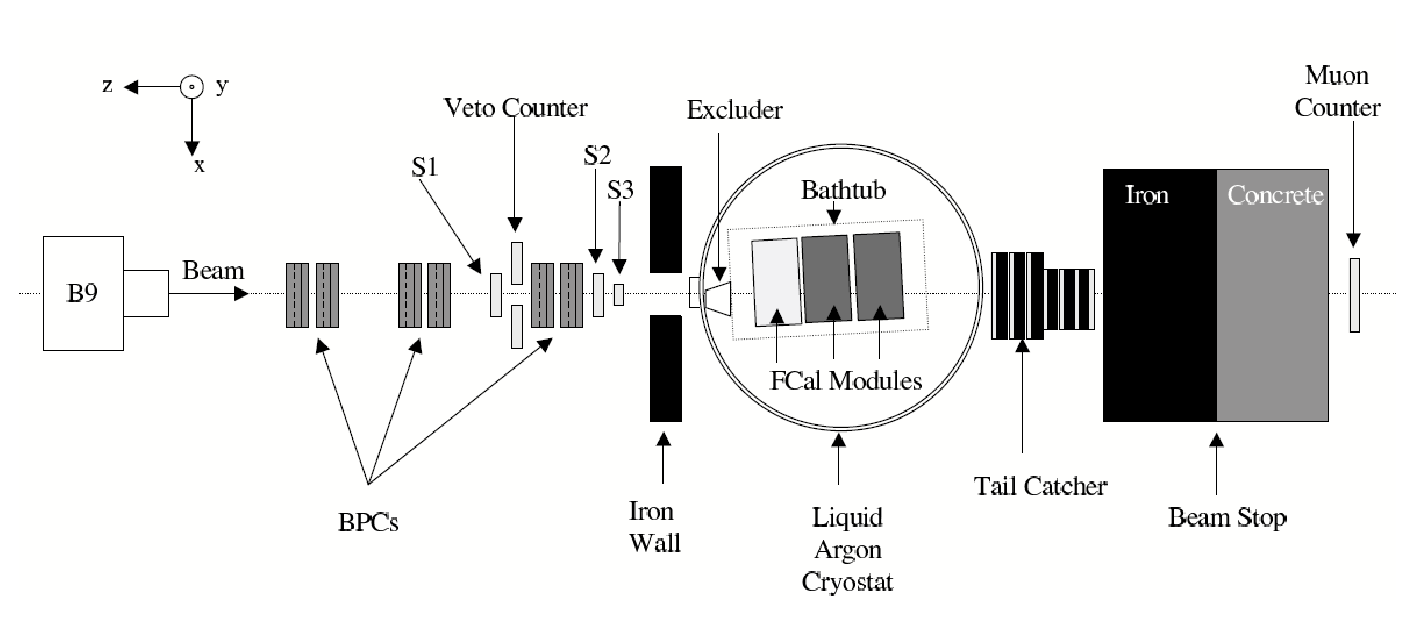
\includegraphics[width=0.8\linewidth,angle=0]{TB_Beamline}
\end{center}
%\centerline{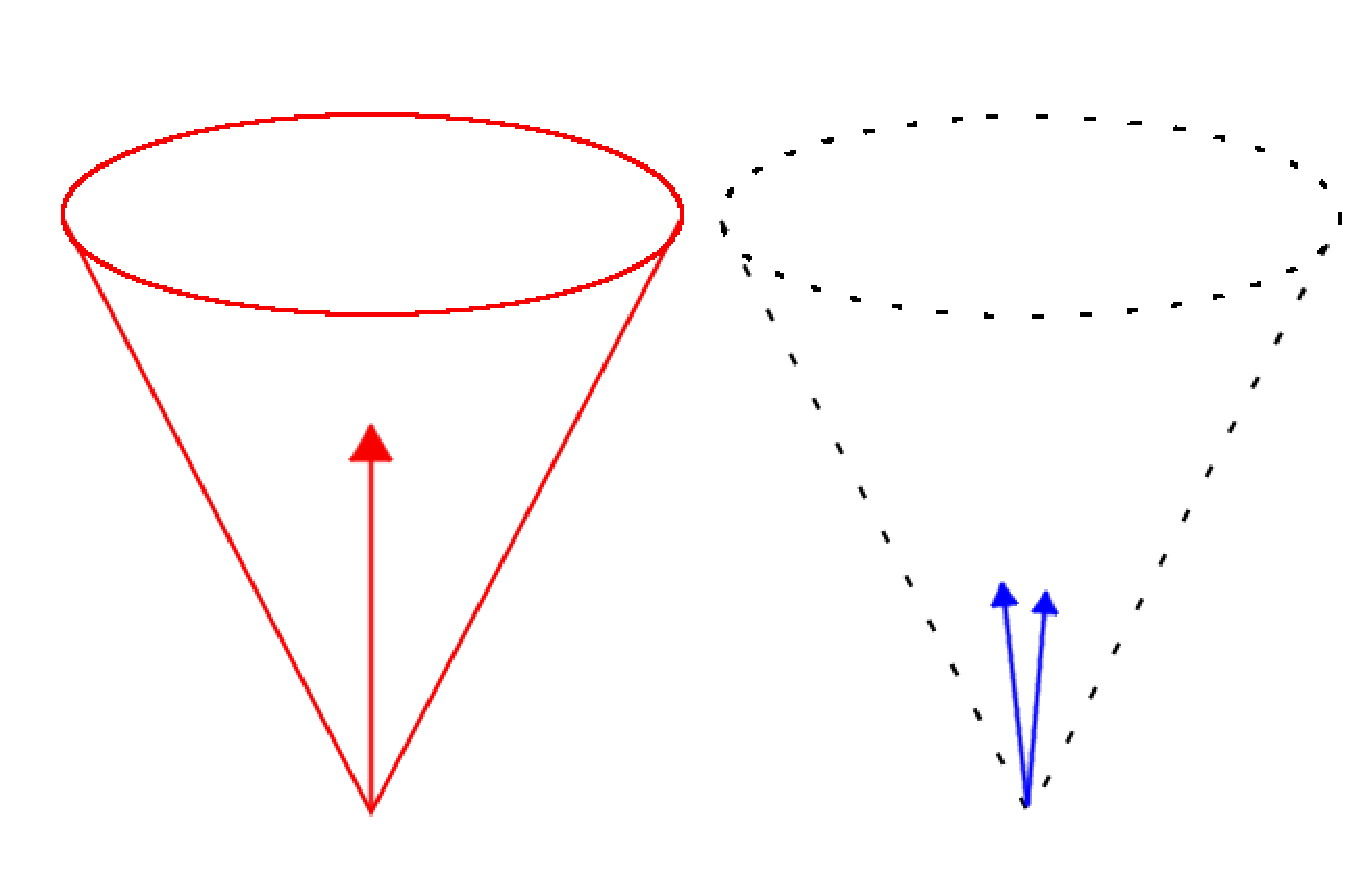
\epsfig{file=./figs/collinear.eps  , width=0.95\textwidth}}
\caption{Diagram showing the setup used for the 2003 FCal beam test (not to scale).}
\label{fig_TB_beamline}
\end{figure}

\begin{figure}[htb]
\begin{center}
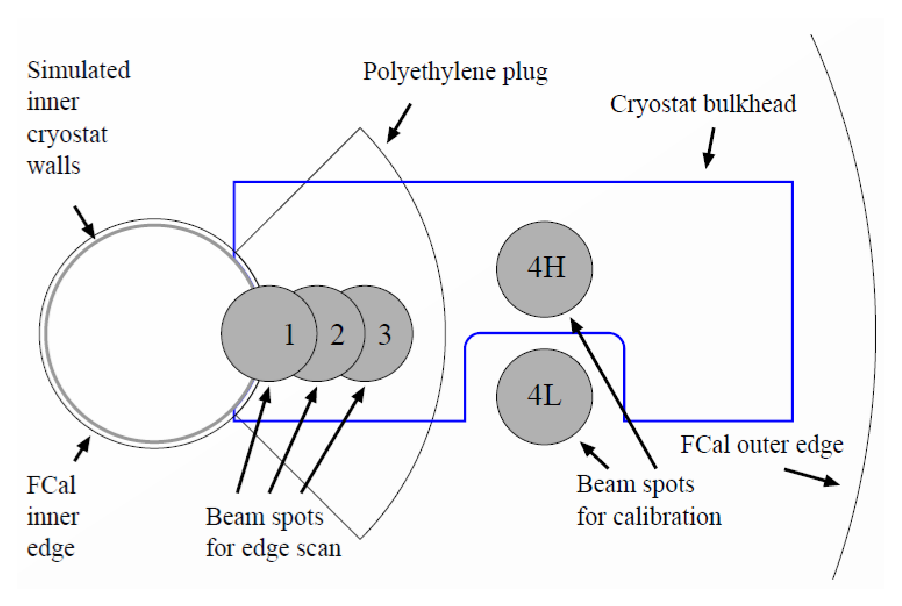
\includegraphics[width=0.8\linewidth,angle=0]{TB_beamspots}
\end{center}
%\centerline{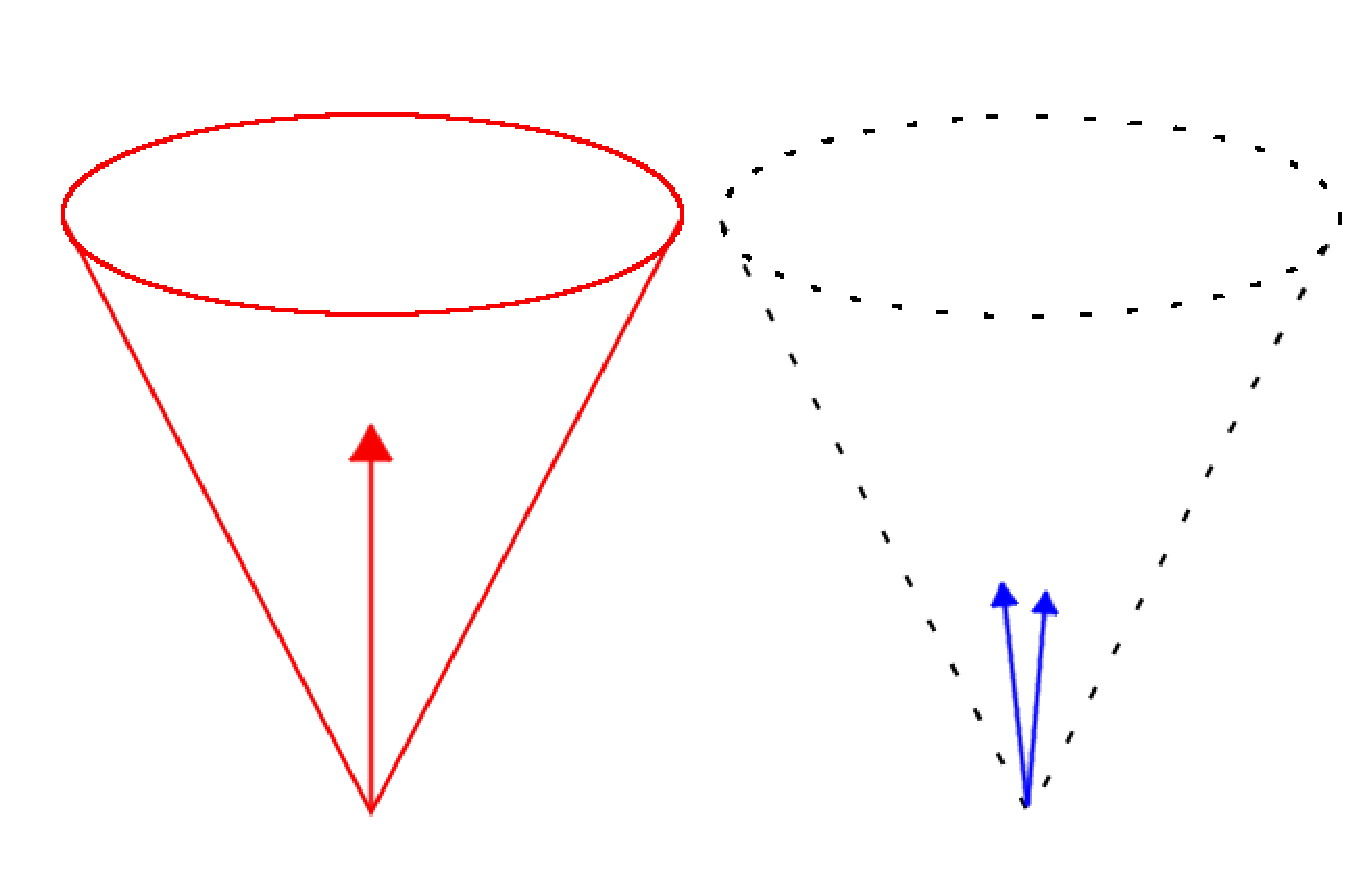
\epsfig{file=./figs/collinear.eps  , width=0.95\textwidth}}
\caption{Beamspots studied in the testbeam.}
\label{fig_TB_beamspots}
\end{figure}

A diagram of the beamline is shown in figure~\ref{fig_TB_beamline}. Beam particles emerge from the B9 magnet, traveling a distance of 32 metres and passing through several sets of instruments before reaching the FCal. The B9 magnet was used to control the vertical inclination of the beam, and thus the vertical position of the beamspot on the FCal face could be controlled via manipulation of the currents in the B9 magnet. The cryostat containing the FCal was able to be translated horizontally and rotated, which provided control over the horizontal position of the beamspot and the angle at which the beam particles struck the front face of the calorimeter. A total of 5 beamspots were used, numbered 1,2,3, 4L and 4H. The locations of these beamspots are depicted in figure~\ref{fig_TB_beamspots}. Positions 1,2 and 3 were used to study the effects of energy leakage down the beampipe from particles impacting close to the inner diameter. High energy ($\sim$200 GeV) beams of electrons and pions were used to provide data at these positions, and the results of these studies can be found in \cite{LouiseThesis,TB03_tbp}. Position 4L was used to study the intrinsic response of the FCal with a minimal amount of material between the calorimeter and the incoming particles, whereas position 4H was used to simulate a more \atlas-like environment with additional dead material introduced into the beamline. Electrons and pions at energies from 10-200GeV were used at these beamspots. This thesis will focus on the analysis of data taken at positions 4L and 4H, and the comparison of this data to results obtained from Monte Carlo simulations.
 



\section{Beamline Instrumentation}
%beam instrumentation and upstream material 
\label{sec_TBoverview_beamline}
\cmt{bpcs: positioning or profile? positioning in FCal paper}
Eight beam positioning chambers (BPCs) were used to provide tracking information on beam particles.
Four of these BPCs were of a more sophisticated design, one pair of which was located about 1.6 metres downstream from the B9 magnet while the other pair was situated 3m upstream from the FCal, on an adjustable table described below. These chambers each contain two readout planes, oriented at right angles such that measurements of both transverse coordinates may be made. Each readout plane covers an area of $120mm \times 120mm$, and has an average resolution of around $130 \mu m$. The other four BPCs were of an older design and were able to measure a single track coordinate with a resolution of about $325 \mu m$. These were positioned in the middle of the beamline (about 20m from the FCal), with two BPCs measuring the X coordinate of the beam particles and the other two the Y coordinate. In total, the eight BPCs provide six independent measurements of the X and Y coordinates of the beam particle tracks.

%\red{should talk about alignment here, or in results}
A mapping between BPC and calorimeter coordinates was established through analysis of electron data. The track measured by the BPCs was projected on to the calorimeter in order to obtain the beam impact point in the BPC coordinate system. This was then associated with the barycentre of the energy deposited in FCal1 using the calorimeter coordinate system. However, the finite granularity of the calorimeter readout tended to bias the position of the energy barycentres towards the centre of the readout cells. This was corrected for by considering the ratio $E_\mathrm{max}/E_1$, where $E_1$ was the total energy deposited in FCal1 and $E_\mathrm{max}$ was the largest energy value contained in a single channel. This ratio was plotted as a function of (BPC) $x$ and $y$, with minimal values in the ratio corresponding to cases where energy was shared evenly between multiple channels. The positions of the minima could thus be associated with cell boundaries in the calorimeter coordinate system, which then allowed the mapping between BPC and calorimeter coordinate systems to be determined with greater precision.
%
%
%Emax - max channel energy
%E1 - total FCal1 energy
%scan accross cell boundaries. 



The adjustable table was positioned about 2 metres upstream from the cryostat, on which three scintillators (S1, S2, S3) were positioned. These scintillators were polystyrene-based, and were used for triggering and ``beam cleaning'', which is discussed in section~\ref{sec_event_selection}. All three scintillators were 1 cm thick, with S1 and S2 having cross-sectional dimensions of 10cm $\times$ 10cm, while S3 had dimensions 7cm $\times$ 7cm. A veto counter was also present on the table, consisting of rectangular piece of scintillator (63cm $\times$ 63cm $\times$ 5cm) with a circular hole 65mm in diameter that the beam passed through. The height of this table could be varied such that the beam instruments were in the appropriate position for the beamspot under study. 

As the liquid argon gaps in the FCal are much smaller than those used in typical liquid argon calorimeters, FCal channels are susceptible to shorts should any conductive debris find its way into the liquid argon. Because the cryostat was not a particularly clean environment, the FCal was housed inside a ``bathtub'' which sat inside the cryostat. The bathtub was made from stainless steel 1.5 mm thick, and had a rectangular shape. Holes were present on its sides to allow the liquid argon to flow in as the cryostat was filled, but these were covered with a fine mesh to keep any debris out. 

\begin{figure}[h]
\begin{center}
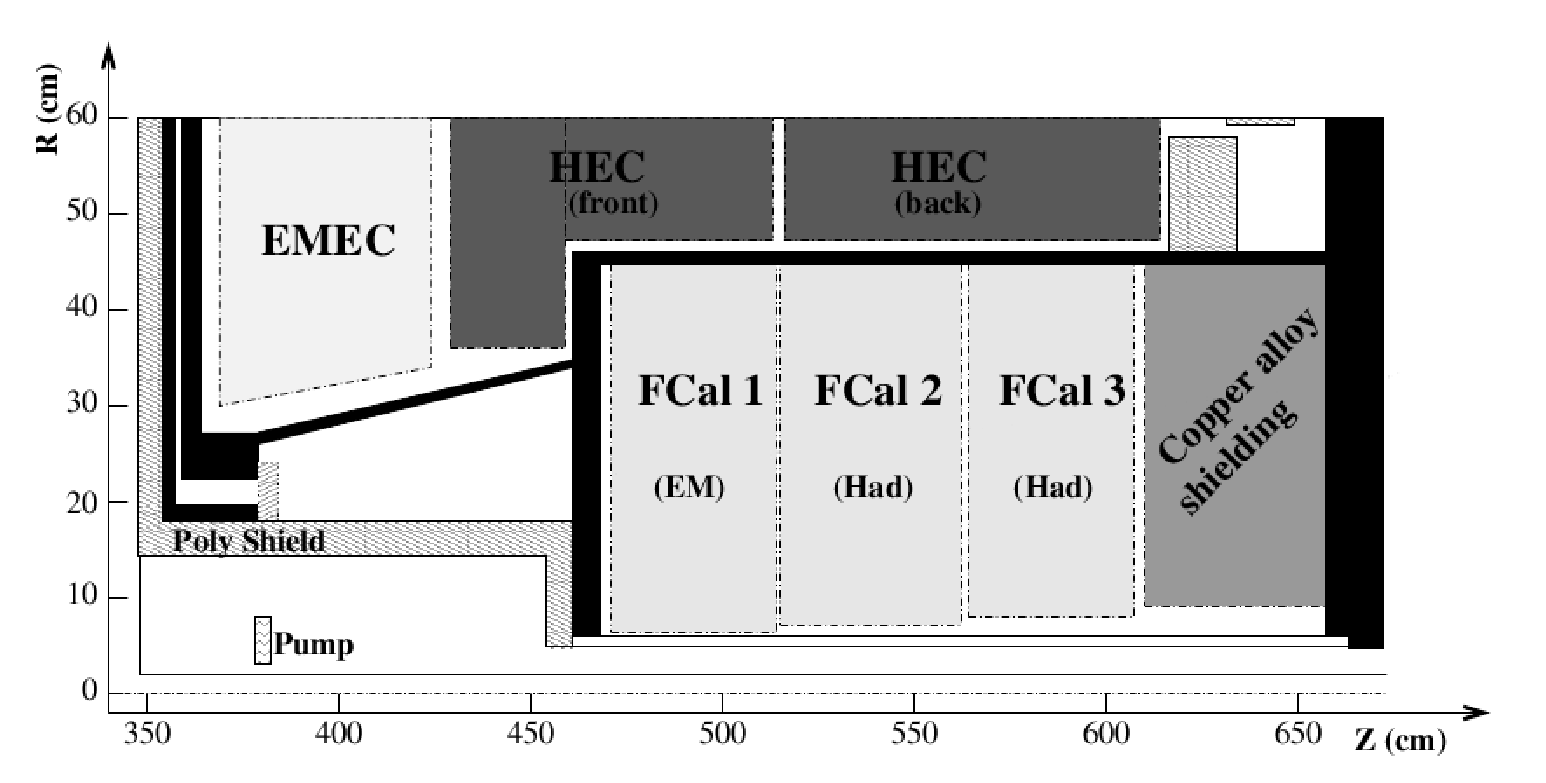
\includegraphics[width=0.8\linewidth,angle=0]{TBoverview/ECxsec_nolines.eps}
\end{center}

\caption{Cross section of FCal positioned within the end-cap cryostat, showing the inactive material laying between the calorimeter and the interaction point. The material in black is associated with the end-cap cryostat.}
\label{end_cap_xsec_2}
\end{figure}

In order to simulate a more \atlas-like environment for data taken at positions 1,2,3 and 4H, additional material was inserted into the beamline. A cross section of part of the \atlas end-cap is shown in figure~\ref{end_cap_xsec_2}, showing the uninstrumented (or ``dead'') material present in the end-cap. An aluminium plate 50.8mm thick was bolted to the inside of the bathtub to model the cryostat bulkhead, with a slot cut out of the plate such that the additional aluminium would not affect beams directed at position 4L. The area covered by this plate is shown in figure~\ref{fig_TB_beamspots}.

The JM shielding (labelled ``Poly Shield'' in figure~\ref{end_cap_xsec_2}) is made of boronated polyethylene and is present in \atlas to prevent albedo radiation from scattering back into the inner detector. This was modelled in the beam test by placing a wedge shaped piece of polyethylene on the outside of the bathtub such that it covered positions 1,2, and 3, simulating the toroidal ``plug'' part of the shielding that lies close to the beam pipe and adjacent to the cryostat bulkhead. An iron wall was located between the adjustable table and the cryostat. This wall had a 10cm x 10cm slot cut into it to allow the beam to pass through. When taking data at position 4H, a rectangularly shaped piece of polyethylene with dimensions 5cm x 20cm x 1m was placed at an angle in this slot. This was done in order to model the tube shaped part of the JM shielding that ran parrallel to the beam axis. When running at position 1, a small piece of aluminium was instead placed in this slot, simulating the ion pump present close to the beampipe in \atlas.

%An ``excluder'' made of RohaCell was also attached to the outside of the bathtub.
In \atlas, there is an evacuated area within the support tube, just in front of the FCal(as shown figure~\ref{}). The support tube used in \atlas was not present during the testbeam, and the FCal was instead mounted on a purpose-built stand within the cryostat. An ``excluder'' made of RohaCell was attached to the outside of the bathtub, in order to prevent the region of space correponding to the evacuated region in \atlas from being filled with liquid argon.
% In \atlas the area between the FCal support tube and the beampipe is evacuated, and so the excluder was placed inside the cryostat to prevent this space from being occupied by liquid argon.
 The density of RohaCell is 0.011 $\mathrm{g}/\mathrm{cm}^3$ whereas that of liquid argon is 1.43 $\mathrm{g}/\mathrm{cm}^3$, so the RohaCell provides a relatively good approximation of a vacuum. A hollow stainless steel cylinder was also placed inside the FCal during the beam test to simulate the beampipe.

A tail-catcher calorimeter comprised of layers of steel and scintillator was positioned downstream of the cryostat. Behind this was a beamstop of iron and concrete, and beyond that a muon counter was located. The tail-catcher and muon counter were only used for muon identification: energy deposited in the tail catcher is not considered when measuring the response of the FCal, or in the derivation of any weights presented in this analysis.

A CEDAR (Cherenkov Differential counter with Achromatic Ring focus, \cite{CEDAR_note}) detector was located upstream of the B9 magnet and used for particle identification. The CEDAR detector consisted of a chamber filled with gas (He) at high pressure. As beam particles passed through this chamber, they would emit Cherenkov radiation at an angle that depended on their velocity and mass. The optics of the CEDAR would then collect this light and focus it into a ring-shaped image, with different types of particles giving rings of different radii. An adjustable annular aperture was positioned in front of a series of photomultipliers, such that they would only detect light from rings of a given radius. The radius selected by the aperture could be tuned such that signal from the photomultipliers corresponded to a beam particle of the desired mass.

% As beam particles passed through a series of chambers filled with gas (He or $\mathrm{N}_2$) at high pressure, and emit Cherenkov radiation at an angle that is dependant on their velocity and mass. The optics of the detector then focus this into a ring, with different types of particles producing rings of differing radii. 

%
%
%
%
%
%
%
%
%\begin{figure}[h]
%\begin{center}
%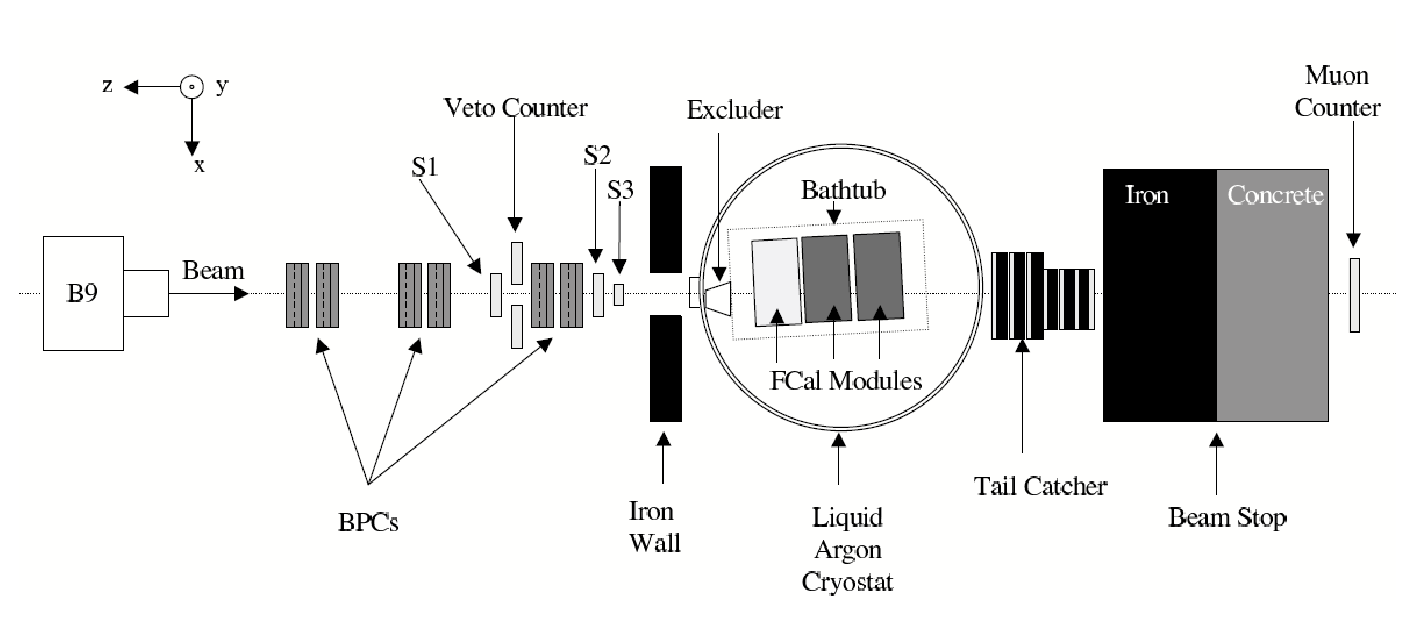
\includegraphics[width=0.8\linewidth,angle=0]{TB_Beamline}
%\end{center}
%%\centerline{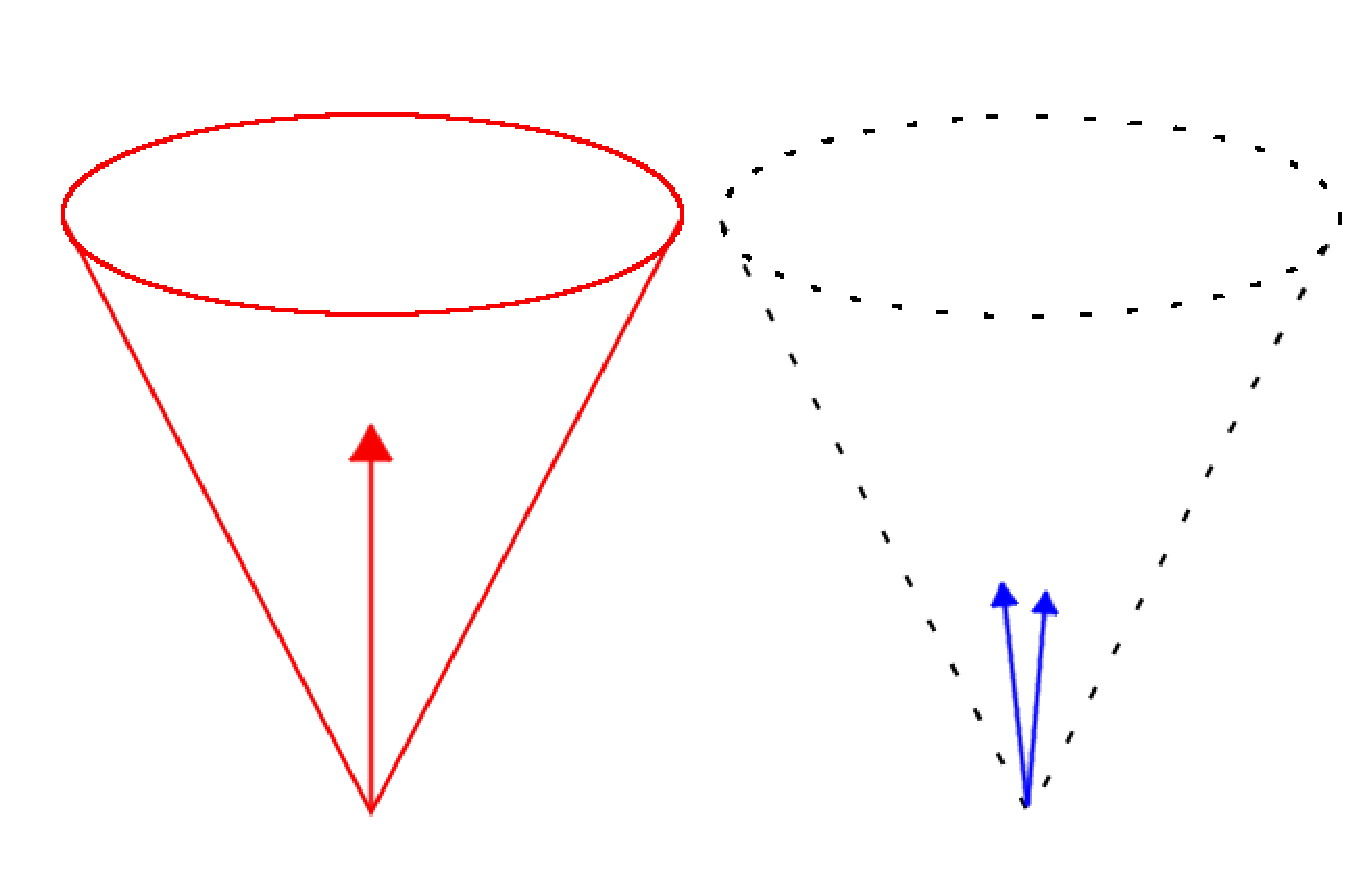
\epsfig{file=./figs/collinear.eps  , width=0.95\textwidth}}
%\caption{Diagram showing the setup used for the 2003 FCal beam test (not to scale).}
%\label{fig_TB_beamline}
%\end{figure}
%
%\begin{figure}[h]
%\begin{center}
%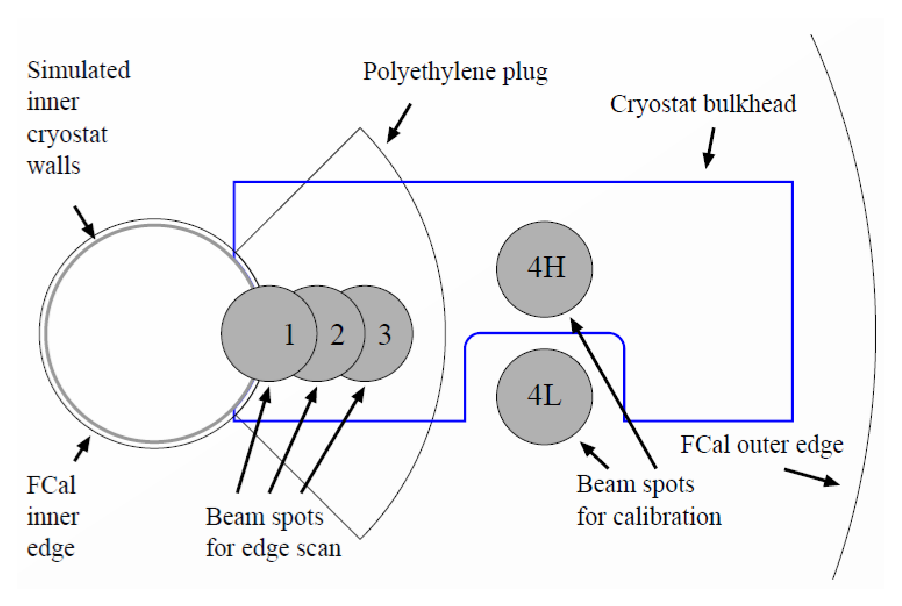
\includegraphics[width=0.8\linewidth,angle=0]{TB_beamspots}
%\end{center}
%%\centerline{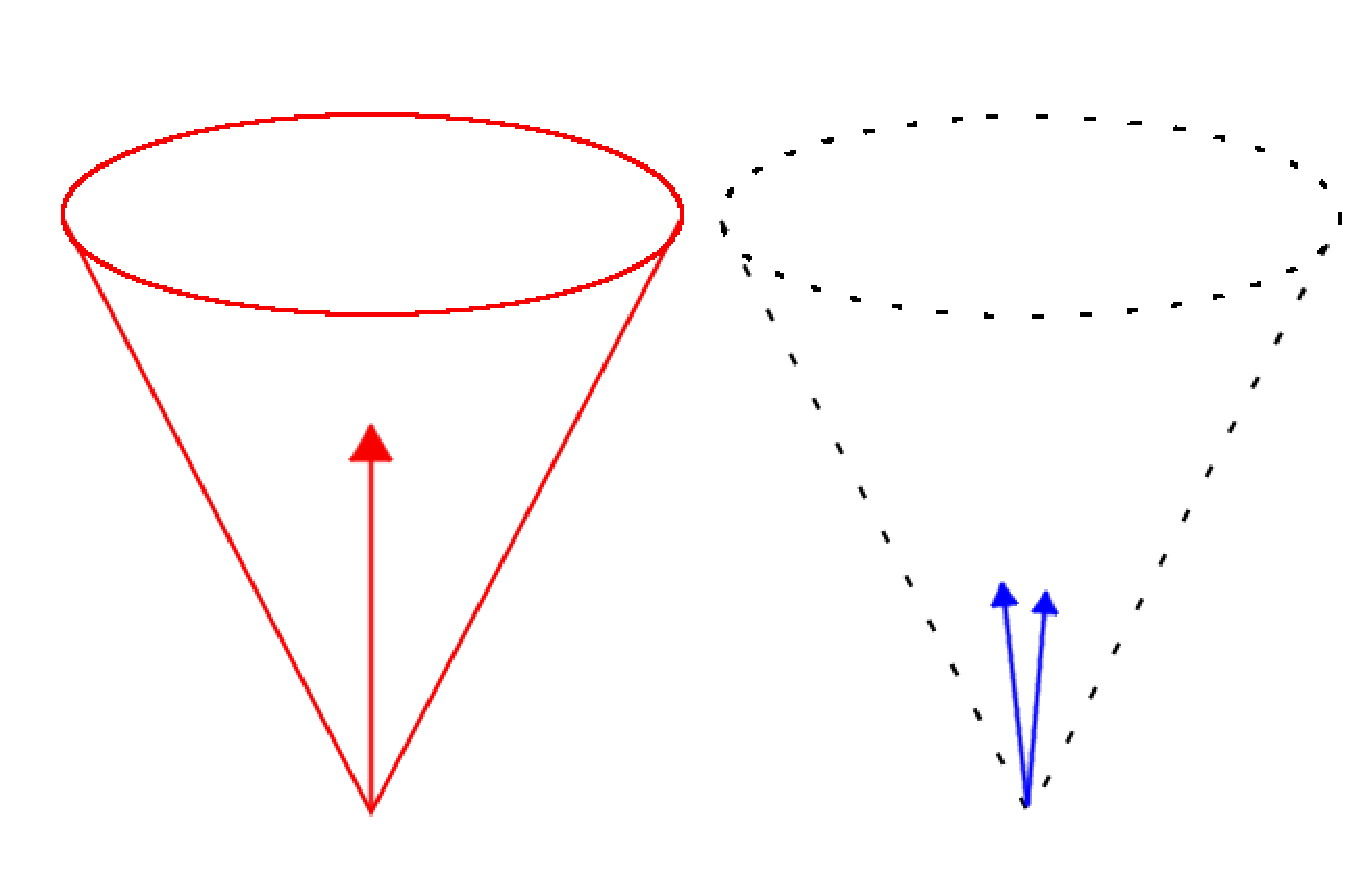
\epsfig{file=./figs/collinear.eps  , width=0.95\textwidth}}
%\caption{Beamspots studied in the testbeam.}
%\label{fig_TB_beamspots}
%\end{figure}
%
%


%
% 
%
% 
%
% Protons from the SPS beam were directed onto targets of in order to produce a secondadary/tertiary beam of the desired particle type.\red{(which targets for which particles?)} . \red{Then a magnet (velocity selector) was used to select particles of the desired type and energy}. 
%maybe skip the details here. secondary/tertiary beam emerges from B9, then stuff happens.
%
%
%
%
%This secondary beam of particles then passed through a bending magnet ("B9"), which controlled the vertical inclination of the beam. The vertical position of the beamspot on the FCal face could thus be manipuilated by varying the currents in the B9 magnet. 
%
%
%The cryostat containing the FCal was positioned 32 metres away from the B9 magnet. The 
%
%
%
%Six Beam Profile Chambers (BPCs) are used to obtain information on the trajectory of the beam particles. The 
%
%BPCs
%
%table scintillators, veto counter
%
%Iron wall, upstream material
%
%Cryostat
%aluminium plate, excluder
%bathtub
%FCal
%
%Tail Catcher
%
%
%\red{move FCal electronics and LAr signal reconstruction to Detector chapter. Keep Timing and offline reconstruction here.}



\subsection{Timing and Pulse Shapes}
\label{sec_TBoverview_timing}
%done using ofc method described in section~\ref{sec_signal_rec_OFC}.\cmt{\red{Test beam studies pulse shapes\ldots}} 
Reconstruction of the calorimeter signal was carried out using the OFC method described in section~\ref{sec_signal_rec_OFC} A SPICE \cite{SPICE_paper} simulation of the electronics chain was used to obtain an initial estimate of the pulse shape used in the OFC calculation. This estimate was then improved using an iterative procedure that incorporated data taken from physics runs. The data used in this procedure was taken from events in which the signal pulses had large amplitudes, in order to ensure that the signal was coming from a physical energy deposit.

Pulse shapes were sampled in time with the TTC clock on the FEBs (described in section~\ref{sec_FCal_electronics}). Seven samples were recorded for each pulse during physics runs, with the timing adjusted such that, on average, the fourth sample was coincident with the pulse peak. In \atlas the timing is synchronised to the LHC clock, such that samples are taken in time with each bunch crossing. This was not the case during the beam test, as beam particles arrived at random phases with respect to the TTC clock. In this case, timing for the event was taken from the S1 scintillator. A LeCroy 2228A Time to Digital Converter (TDC)  with a timing resolution of 50 ps was used to measure the phase difference between the event trigger and the TTC clock, with the trigger from the S1 scintillator used as a start signal and the clock pulse from the TTC used as a stop signal. The TDC only measured a phase difference between the start and stop signals, and so readings close to 0 or 25 ns were ambiguous. To resolve this a second TDC was used in which the stop signal was delayed by 10 ns, which allowed the time interval between the beam trigger and the TTC pulse to be determined uniquely. 

While the OFC method is capable of handling time differences between pulse peaks and sample times, the Taylor expansion used in equation \ref{eq_OFC_taylor} becomes invalid when this time, $\tau$, becomes large. To avoid this issue, events are binned according to the TDC phase time, using 25 bins of width 1 ns. A set of OFCS is calculated for each bin using a pulse shape that has been shifted in time by the relevant amount. During event reconstruction, the amplitude of each pulse is obtained by using the set of OFCs corresponding to the TDC phase time for that event. Only a single set of OFCs is required at \atlas, as in this case the TTC clocks are synchronised with that of the LHC, and so the samples are taken in time with the bunch crossings.

%
%For each of the 25 bins, a set of OFCs are calculated using a pulse shape shifted in time by the relevant amount. During signal reconstruction, the TDC phase time is used to look up the correct set
%
%
%
% 
%
%A SPICE simulation of the electronics chain is used to obtain an initial estimate of the pulse shape used in the OFC calculation. This estimate was then improved using an iterative procedure that incorporated data taken from physics runs. 
%
%To avoid this issue, 
%
%%The pulse shapes used in deriving the OFCs are taken from physics data, using events which had a large peak and were thus due to physical energy deposits.
%A SPICE simulation of the electronics chain is used to obtain an initial estimate of the pulse shape used in the OFC calculation. This estimate was then improved using an iterative procedure that incorporated data taken from physics runs.   
%
%
%The samples were fitted to a pulse shape prediction obtained through simulation of the electronics chain in order to find the time and amplitude of the pulse peak. Each pulse was then shifted and scaled so that the peak occured at time zero and had unit height. 
%
%
%
%
%
%
%OFC calculation.
%
%
%
%
%
% TTC every 25 ns.
%S1 random with respect to this, so LeCroy TDC used to measure time shift/phase between TTC and S1 with 50ps resolution. Second TDC used to remove phase ambiguity at 0/25 ns (are things exactly in time or 25ns off?) 
%
%because things arrive asynchronously, OFCs computed for 1ns bins of phase difference, i.e. 25 different sets of OFCs derived. timing phase used to select OFCs used for signal reconstruction.
%
%Pedestal - physics triggers, first (of seven) sample used for pedestal studies. Pedestal subtracted from pulse. 
%
%Pedestal value calculated for each channel, run by run. Noise for each sample taken as RMS of pedestal - 3.2 ADC on average.
%
%random trigger data used for noise autocorrelation?
%
%
%
%
%
%
%
%
%
%
%

\subsection{Offline Reconstruction}
\label{TBoverview_offline}
Offline reconstruction of testbeam data is carried out in \athena. A flowchart depicting the data structures and algorithms used in the reconstruction of data and simulation events is shown in Figure~\ref{TB_data_flowchart} For each event, the LArRawChannelBuilder algorithm retrieves the pulse samples (which are stored as LArDigits), and fetches the OFCs from a database. The pedestal is then subtracted from these samples and the OFCs are applied, giving the amplitude of the pulse in ADC counts. This amplitude is then converted to an energy using a factor (the ``ADC2MeV'' value) that depends on the channel and gain. The energy of the channel, in MeV, is then stored as a LArRawChannel object. Another algorithm is then used to create  CaloCell object from this LArRawChannel. From the CaloCell the position, time, energy, quality, and four-momentum of the channel may be retrieved, making CaloCells suitable objects to be used in data analysis. Because of this, CaloCell information is recorded by default in Event Summary Data (ESD) files, which are one of the standard formats used by \atlas. CaloCells are also used as input for topoclustering algorithms, which in turn are used as input for jet-finding and missing energy algorithms.

For initial studies of the testbeam data, the ADC2MeV factors used in the reconstruction were set to 1, so that the final energies were obtained in terms of ADC counts. This was done so that the actual ADC2MeV values could be extracted from the data more easily. However, the LArRawChannel class used in \athena stores channel energys as an integer number of MeV, as energies less than 1 MeV are deemed insignificant. An unforeseen consequence of this was that in earlier versions of the testbeam analysis, cell energies were truncated (rounded down) to an integer number of ADC counts. This rounding meant that energy was effectively lost during the reconstruction proccess, up to $\sim$80 MeV per cell in FCal1 and $\sim$160 ($\sim$185) MeV in FCal2 (FCal3). This had some effect on the electron results but a more significant effect on the hadron results, due to broader showers and higher ADC2MeV factors associated with the hadronic modules. The bug has since been fixed, and none of the results presented here are affected by it.


\begin{figure}[h]
\begin{center}
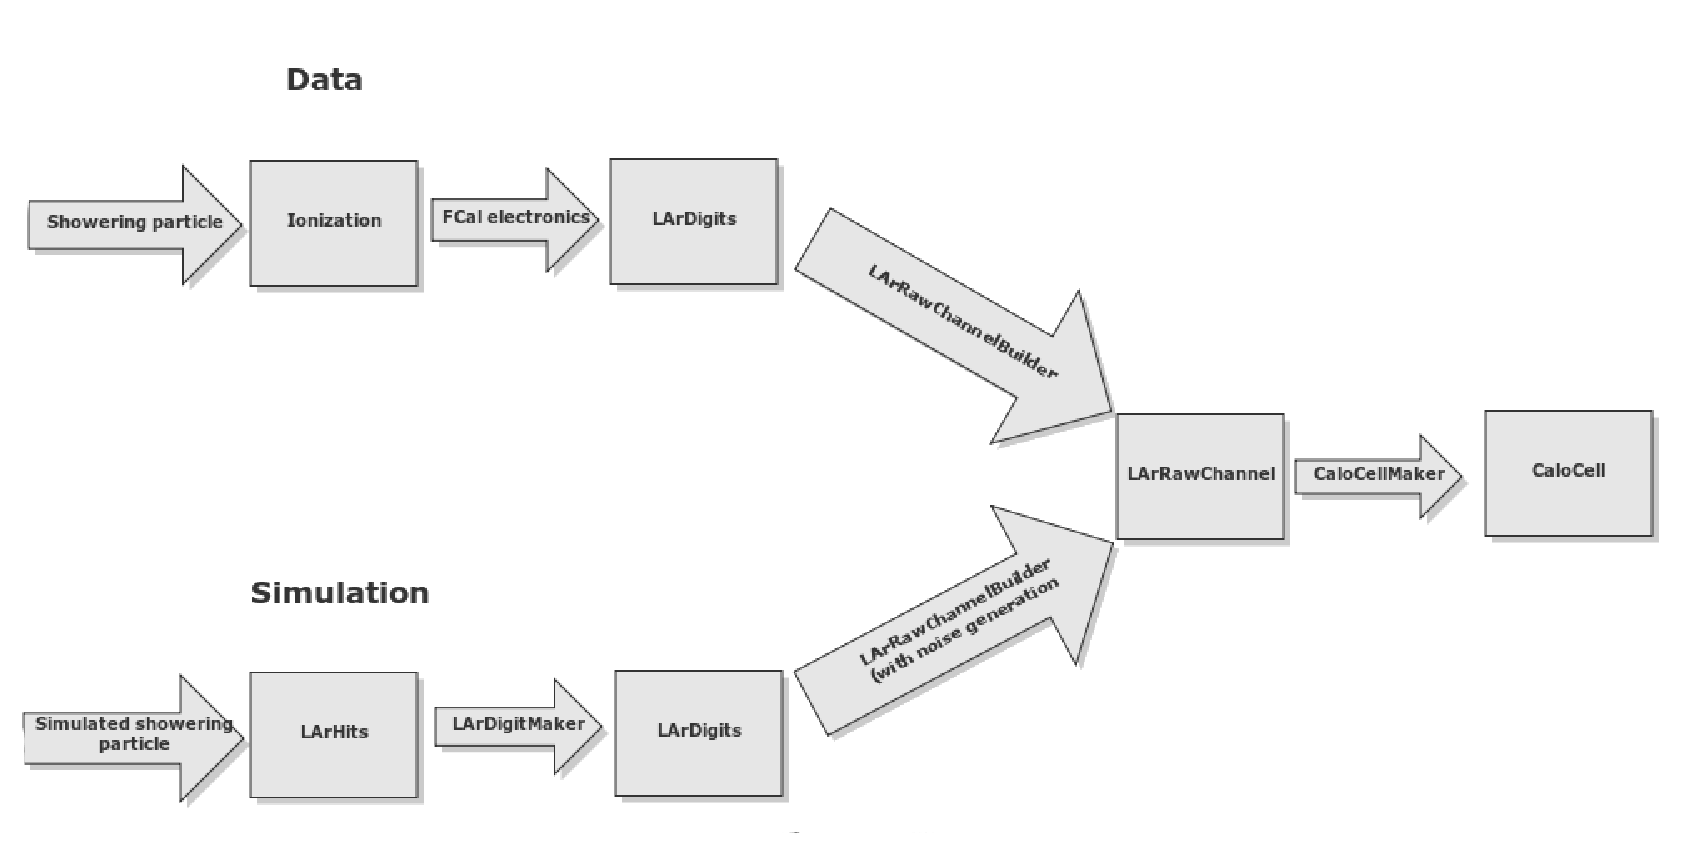
\includegraphics[width=0.9\linewidth,angle=0]{TBoverview/TB_data_flowchart.eps}
\end{center}

\caption{Flowchart showing the processes/algorithms and data structures involved in the reconstruction of testbeam data and simulation results.}
\label{TB_data_flowchart}
\end{figure}

\section{Monte Carlo Simulation}
%\subsection{Monte Carlo}
%\subsection{reconstruction}
%\subsection{noise}
%athena/G4/geometry
%digi/reco
%noise


A Monte Carlo simulation of the testbeam setup has been developed within the \athena framework. \cmt{The simulation describes all elements of the beamline from the B9 magnet to the tailcatcher.} Geant 4.9.2 \cite{geant4} is used to simulate interactions of the beam particles with beamline elements. The results of this simulation are then reconstructed and analyzed in the same manner as the data.

\subsection{Geant4 Simulation of the Forward Calorimeter and Testbeam Environment}
\label{TB_overview_g4}
Geometry in \geant is described in terms of volumes. A ``solid volume'' is first created to describe the shape of a given object. This is then used to derive a logical volume, which inherits the shape of the solid and is associated with a material. A material type is defined by specifying the relative mass fractions \cmt{of the elements of which it is composed} of its constituent elements and the density of the material. Logical volumes are then used to construct physical volumes \cmt{(PhysVols)}, which inherit the shape and material information from the logical volume. A physical volume also has a position and orientation assigned to it, and it is by positioning these physical volumes that the geometry of the simulation is defined. A special physical volume, the world volume, is created first. All subsequent physical volumes are then placed either inside the world, or inside another physical volume. 
%The position and orientation of a physical volume are specified through transformations: rotations and translations. A physical volume is placed at the origin of the volume it is inserted into, and transformation operations are then applied to reposition it. 

The description of the beamline used in the simulation contains all the beamline elements from the B9 magnet to the tailcatcher, including all scintillators, BPCs, cryostat material and beampipes. Most of these objects are defined from scratch, however the description of the FCal is taken from that used in the full \atlas simulation while the cryostat description has been taken from another testbeam simulation. Elements upstream of the B9 magnet, such as the CEDAR detector, have not been included. 

The description of the FCal has been modified in some respects, to improve some aspects of the material description. In the default FCal definition the rods in the hadronic modules are made of WFeNi whereas they are actually pure tungsten, which has a slightly higher density. The density of the absorber matrix was also corrected, as an updated estimate of this value was obtained. The correct materials and densities (given in section~\ref{chap_Detector_FCal}) have been used in the testbeam simulation.

%The abstract way in which positions are defined can also lead to errors. \geant uses matrices to represent transformations, and so the order of operations are important. When a physical volume is inserted into the world (or another physical volume), it is placed at the origin of that volume's coordinate system, and must be repositioned by applying transformations. These transformations are not commutative, so care must be taken to ensure the operations are applied in the correct order. The last operation specified prior to the creation of a physical volume is the first operation applied to it once it is placed in the world, which can be counterintuitive if these transformations are not thought of as matrix operations. 

%For example, the Cryostat description takes the z axis to be vertical, whereas in the geometry used by \atlas and the testbeam the z axis is the beamline (i.e. horizontal). The cryostat is thus rotated $90^\deg$ before being inserted into the world. Consequently, the 

In \geant, physics is defined in terms of processes. Particles are propagated through the simulation in a step by step fashion, with continuous processes (such as ionisation) acting on the particle during the step while discrete processes (such as decays, pair production) take place at the end of a step. After each step, the particle's kinematics are updated. Secondary particles are only produced if their energy exceeds a ``range cut''. If a process would produce a secondary particle with energy less than the range cut, this energy is instead deposited in the material. Range cuts are specified as a distance, but \geant converts this distance to an energy based on the material the particle is travelling through at the time. A range cut of $30 \mu m$ has been used for testbeam simulations, which is appropriate given the narrow width of the active liquid argon gaps. In the full \atlas simulation, range cuts of 100$\mu$m are used in the EM barrel and EMEC calorimeters, while a cut value of 1mm is used in the HEC. The full \atlas simulation also uses a range cut of $30 \mu m$ for the FCal.

%Interactions of particles with matter are done in a step by step manner. At each step, particles in the simulation are moved forward by an amount dependant on their kinematics and any physical processes that may be relevant.  
%
%http://geant4.web.cern.ch/geant4/UserDocumentation/UsersGuides/ForApplicationDeveloper/html/ch05.html#sect.Track
%
%Electromagnetic showers only consist of a relatively small number of  processes (e.g. Bremstrahlung, pair production, ionisation), and so are relatively straightforward to model.

Electromagnetic showers are generally well understood and relatively straightforward to model. Hadronic showers are more complex, and a variety of processes are used to describe the shower development. Hadronic ``physics lists'' are used to define the specific set of processses available and the energy ranges in which they are used. Three physics lists have been used in the simulation of the test beam, and are outlined below:

\begin{itemize}
\item{QGSP-BERT:} Quark Gluon String Precompound with Bertini cascade. This is the default physics list used for \atlas simulations. The Quark Gluon String model \cite{QGSP_paper} is used to simulate hard inelastic scattering for hadrons in with energies from 12 GeV to 100 TeV. One or more strings are formed between between partons of the colliding hadrons, and these strings are then ``cut'' by inserting quark/anti-quark pairs. One member of the pair becomes the new ``end'' of the string, while the other forms a hadron with the parton that was the old end. This process repeats until the string has insufficient energy to form new pairs. The precompound model is then used to de-excite what remains of the nucleus.
Between 9.5 and 25 GeV, a Low Energy Paramaterization (LEP) is used to describe inelastic scattering \cite{LEP_paper}. 
For particles with energy less than 10 GeV, a Bertini intra-nuclear cascade model \cite{ Bertini_paper, Bertini2} is used to describe inelastic scattering with nuclei. The incoming hadron is classically scattered within the nucleus, using cross sections and angular distributions taken from experiment. 
\item{QGSP-BERT-HP:} This physics list is essentially the same as QGSP\_BERT, but includes high precision modeling for low energy neutrons ( $<$20MeV). This method relies extensively on cross sections obtained from experiment. It was reported in \cite{QGSP_HP_note} that the high precision neutron tracking had a significant effect on the development of hadronic showers in tungsten, and so it was considered worthwhile to investigate this physics list.
\item{FTFP-BERT:} This physics list uses the Fritiof string model \cite{Fritiof_string_paper} to model high energy inelastic interactions, which is similar to the Quark-Gluon String model described above. The Fritiof model can be applied over a wide range of energies, and is used for hadrons with energies between 4 GeV and 100TeV. As with QGSP\_BERT, the precompound model is used to de-excite the nucleus following the Fritiof interaction. The Bertini Cascade model is also used at energies below 5 GeV.
\end{itemize}





%geometry - uses volumes. solid volumes for shape logical volumes for material/density,  physical for position within world.
%
%positioning carried out through transformations - translations and rotations. physical volumes placed within physical volumes.
%
%Some parts FCal, "based of descriptions used..."taken from \atlas or other simulations of beam tests of other detector components.
%need to be careful here. small errors were found in the densities and materials used in default \atlas simulation. For example, the rods used in the default simulation are made of WFeNi material rather than pure tungsten, which is of a slightly higher density. The density of the default absorber matrix was also found to be too high/low, whereas the correct value (14.39g/cm3, c.f. section XX) has been used in the testbeam simulation.
%
%Abstract way in which positions are defined can also lead to errors. Transformations (translations/rotations) are defined in terms of matrices, and the order of operations are important. When a physical volume is inserted into the world (or another physical volume), it is placed at the origin of that volume's coordinate system, and must be repositioned by applying transformations. These transformations are not commutative, so care must be taken to ensure the operations are applied in the correct order. The last operation specified prior to the creation of a physical volume is the first operation applied to it once it is placed in the world, which can be counterintuitive if these transformations are not thought of as matrix operations.
%
%The representation of the cryostat takes z direction as being vertical, whereas \atlas and the beam test use z to be the beamline. This kinda fucks everything up.
 
%Interactions of particles with matter (i.e. physical volumes) are carried out in a step by step fashion. 
%How does G4 work, exactly?
%
%kinematics ->get step size from processes
%move by the step
%update kinematics (all active processes used
%maybe decay?
%continue
%
%particles tracked untill they have no energy, but not produced unless they have enough energy to travel a certain distance, range cut.
%
%Electromagnetic showers pretty straightforward, consist of a few processes. Hadronic showers more complex, and various processes/models are used in the shower development. A Hadronic physics list is used to define the specific set of processes available and then energy ranges in which they may be used. Simulations have been run using the three physics lists described below
%
%QGSP\_BERT quark Gluon String Precompound with Bertini cascade QGString, fragments, interacts with precompund. Bertini used at lower energy
%
%FTFP\_BERT Fritiof string model, with bertini
%
%QGSP\_BERT\_HP. like QGSP\_BERT, but uses tables of data from neutron scattering. Investigated this physics list after it was noted in \cite{} that slow neutrons are important for showers in tungsten. generally gives results similar to QGSP\_BERT, but takes a lot longer to run.
%
%%http://geant4.cern.ch/support/proc_mod_catalog/physics_lists/hadronic/FTFP_BERT.html
%%http://geant4.cern.ch/support/proc_mod_catalog/physics_lists/hadronic/QGSP_BERT.html
%
%hits - showering particles deposit energy via ionisation in active region (LAr Gaps of FCal), information is stored as a G4 hit from which the energy, time, and location of the deposited energy can be accessed. A vector of these hits is stored for each FCal channel, and used as an input for the reconstruction. 
%%If desired, calibration hits can also be enabled, in which case information is stored for energy deposited in dead/inactive areas of the beamline, including the absorbing material of the calorimeters. This is useful for determing the sampling fraction of the calorimeter.






%simulation uses geant 4.9.2 within \athena
%
%geometry - everything in the beamline from the B9 magnet to the muon counter (TC?) - not the CEDAR
%geant 4 uses shapes, logical volumes, physical volumes
%
%processes - particles take steps, looks at available processes, rolls dice and does something.
%
%Hadronic processes and physics lists




%
%mention volumes used, solid defined by shape, logical volume made from a solid, associated with a material. Physical volumes is an instance of a logical volume given a position in the MC "World". Position defined w.r.t world or another physical volume.
% The geometry used in the simulation describes all instrumentation and material from the B9 magnet to the tail catcher calorimeter, covering a length of over 30 metres. Material upstream of the B9 magnet, including the CEDAR detector and large air gaps traveresed by the beam, was not simulated. 
% sell this, over years description has been refined, errors corrected. try to emphasise how complex and abstract geometry definition in G4 is.
% maybe talk about how geometry done, defining solids, logical and physical volumes, transformations, etc.





\subsection{Reconstruction of Simulation Results}
The reconstruction chain used for Monte Carlo simulations is, with a few exceptions, the same as that used for reconstruction of the test beam data. In \geant, when a showering particle deposits energy through ionization in a liquid argon gap, a ``hit'' is produced. The hit describes the size, time and location of the energy deposited in the liquid argon. A digitization step then collects these hits and simulates the electronics chain to in order to produce digitized samples of the pulse shape, which are again stored as LArDigits. These are then processed into LArRawChannels and CaloCells in the same manner as is used for data, as shown in figure~\ref{TB_data_flowchart}.


Electronic noise must also be modeled in the simulation. For the FCal, most of this noise arises in the preamplifiers on the summing boards. Noise can be quantified by studying the rms of the pedestal values, which gives a value of 3.2 ADC counts per sample when averaged over all channels and all runs. In addition to physics data, some randomly triggered events were recorded during data taking. The data taken by these random triggers is essentially all noise, and allows correlations in the noise between channels to be studied.

\begin{figure}[bht]
\begin{center}
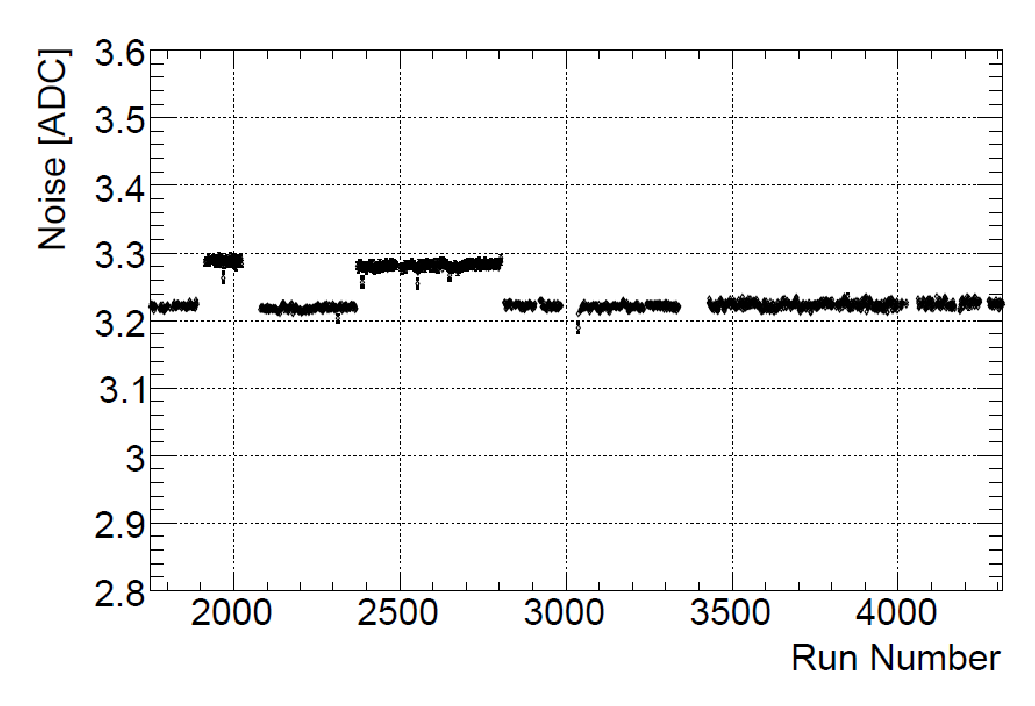
\includegraphics[width=0.8\linewidth,angle=0]{TBoverview/noise_v_run.eps}
\end{center}
\caption{Plot showing variation in the pedestal RMS, as a function of run number. The pedestal RMS is an indication of the level of noise present in the electronics, showing that this varied with time.}
\label{pedestal_variation}
\end{figure}

The default method for modeling noise in the simulation is done during the digitization step, where the autocorrelation matrix for the noise is retrieved from a database. It is then used to randomly generate the noise contributions that are added to each sample. However, during data taking the level of electronic noise present was seen to vary, as can be seen \cmt{the pedestal values }in figure~\ref{pedestal_variation}. Data for different beam configurations was taken at various times, so the average noise present for runs at a specific particle/beamspot/energy differs from that for runs with another beam configuration. 

To account for this, randomly triggered data taken from the same runs as the physics data is used to generate the noise added into the simulation, using a procedure discussed below. This method allows different beam configurations to be reconstructed with different levels of noise, whereas the default method of generating noise lacks this functionality.


%
%
%
%
%
%The default method for modeling this noise is done during the digitization step, where a randomly generated noise contribution is added to each sample. 
%
% The default method for applying this noise is to add a random amount 
%
%The default method for modeling this noise is done during the digitization step, where a randomly generated noise contribution is added to each sample. 
%
%In addition to physics data, some randomly triggered events were recorded during data taking. 
%
%
%Noise can be quantified by studying the rms of the pedestal values, which gives a value of of 3.2 ADC counts per sample when averaged over all channels and all runs. In addition to physics data, some randomly triggered events were recorded during data taking. The data taken by these random triggers is essentially all noise, and allows the correlations between samples to be studied. 
%
%
%
%
%
%Default: noise autocorrelation retrieved from database, which is used to randomly generate the noise that is added to each sample. 
%
%
%However, during data taking the level of electronic noise present was seen to vary, as can be seen from the pedestal values in figure~\ref{}.
%Runs for different beam configurations done at various times, so average noise present for specific particle/beamspot/energy will be different to that for another beam configuration. 
%To account for this, randomly triggered data taken from same runs as the physics data is used to generate noise added into the simulation, using a procedure discussed below. Default method generating noise lacks this functionality.
%
%
%
%
%
%noise observed to vary
%
%
%
%
%after event simulated, reconstruction done the same way as data, with some exceptions
%First, LarDigitMaker used to simulate electronics and turn hits into digits., which are then fed to LarRawChannelMaker.
%second is the way in which noise is handled. noise needs to be simulated in Monte Carlo. By default, this is done in digitization, random amount added to each sample. Testbeam case this is not done, instead the noise is added to the LArRawChannelBuilder algorithm.  

\subsection{Noise Generation and Application}


%As data-taking progressed, the level of noise observed in the FCal electronics was seen to vary from %run to run. \red{cause?}. Data for a different sets of run conditions (beam energy, particle type, beamspot position) taken with different level of noise present. 
%
%The RMS of the electronics noise over all runs is 3.2 ADC counts per sample for summed channels \red{and unsummed attenuated channels}. The simulation initially used this value when modeling the electronics noise during the digitization process, by adding or subtracting a random amount to each sample. However, as the level of the noise varied during data taking it was decided that the simulation should model this, and that the noise used in the simulation should reflect the noise present in the data.
%
%For a given set of data, e.g. 200GeV electrons at position 4L, data taken from randomly triggered events is used to calculate the properties of the electronics noise and model this in the simulation. The random data is used to generate a covariance matrix, describing the correlations between channels


The noise added into the simulation is derived from the randomly triggered data. A covariance matrix is generated by running over the randomly triggered data taken with a specific beam configuration (e.g. 200GeV pions directed at position 4L), such that 
\begin{equation}
M_{ij} = \frac{1}{N_\mathrm{events}}\sum_n^{N_\mathrm{events}} e_{i,n} \, e_{j,n}
\end{equation}
where $e_{i,n}$ is the noise reconstructed from the $i$-th channel of the $n$-th event, in ADC counts. The matrix $M_{ij}$ is then diagonalised, such that it can be written as
\begin{equation}
\mathbf{M} = \mathbf{U}^T \, \mathbf{D} \, \mathbf{U}
\end{equation}
where $\mathbf{U}$ is a unitary matrix with columns equal to the eigenvectors of $\mathbf{M}$, and $\mathbf{D}$ is a diagonal matrix which has the eigenvalues of $\mathbf{M}$ as its entries. The matrix $\mathbf{U}^T$ thus acts as a transformation matrix, transforming information from the ``channel'' basis to the eigenvector basis. The eigenvectors and eigenvalues are written to file, and then retrieved during the reconstruction.

The noise is applied in the LArRawChannelBuilder algorithm, after the pulse peak has been found through application of the OFCs. \cmt{sensible, as this method makes no use of information on individual samples.}The matrix $U_{ij}$ and eigenvalues $D_{ii}$ are first read from file. For each event a vector of noise, $N_i$ is then generated. This is done in the eigenvector basis using a normal distribution, such that $sigma (N_i) = D_ii$. This noise is then transformed back into channel basis, such that 
\begin{equation}
N^\prime_i = \sum_j U_{ij} \, N_j
\end{equation} 
which builds in all the correlations between channels. The noise $N^\prime_i$ is then added to the reconstructed pulse peak of the $i$-th channel.

The default method relies on an autocorrelation matrix, such that a correlations between samples are present but each channel is considered independently. The alternative method described above avoids dealing with the noise on individual samples and instead considers the total noise on the reconstructed pulse peak, while also incorporating correlations in the noise between different channels. These correlations are significant, as without them the estimations of the noise contribution in a given cluster are too low. This is important when studying the energy resolution of the FCal, which will be discussed later.


%
%
%
%
%
%
%
%
%
%
%
%
%store eigenvectors and eigen values. (check this).
%
%in ChannelBuilder, vector of noise generated in eigenvector basis. This vector is then multiplied by matrix of eigenvectors in order to transform back into the channel basis. noise then applied to each channel.
%
%method ensures that correlations in noise between channels are preserved, which does not happen in default method. Initial attempts at implement noise only focused on using the correct RMS for each channel, neglecting correlations. Clustered noise was subsequently found to be too low.
%
%
%
%diagonal
%
%   



